
%%==================================================
%% demo.tex for BIT Thesis
%% modified by yang yating
%% version: 1.2
%% last update: Jan. 4th, 2018
%%==================================================

% 默认单面打印 oneside 、硕士论文模板 master

\documentclass[oneside, master]{BIT-thesis-grd}

% 模板选项: 硕士论文 master; 博士论文 doctor

%==============更改数学字体设置,Latin Modern Math 默认的的确有点细,看个人需要,下面提供一种方法,需要的可以取消注释=========%
\usepackage{url}
\usepackage{float}
\usepackage{amsmath}
\nocite{*}
\usepackage{multirow}
% \usepackage[bold-style=ISO]{unicode-math} %采用unicode-math,可以直接输入Unicode公式,当然传统的输入就行
% \setmathfont{XITS Math}  %目前unicode-math 支持几种数学字体,具体用法可以查看帮助文档,这里采用类似times字体科学数学字体,可以取消注释对比


\begin{document}
%%%%%%%%%%%%%%%%%%%%%%%%%%%%%%
%% 封面
%%%%%%%%%%%%%%%%%%%%%%%%%%%%%%

% 中文封面内容(关注内容而不是表现形式)
\classification{TQ028.1}
\UDC{540}

\title{面向代码克隆检测的多维源代码表征学习方法研究}
\vtitle{面向代码克隆检测的多维源代码表征学习方法研究}
\author{王丹}
\institute{计算机学院}
\advisor{马锐副教授}
\chairman{**教授}
\degree{工学硕士}
\major{计算机技术}
\school{北京理工大学}
\defenddate{2024年5月}
%\studentnumber{**********}


% 英文封面内容(关注内容而不是表现形式)
\englishtitle{Research on Multidimensional Source Code\\Representation Learning Method for Code Clone Detection}
\englishauthor{Wang Dan}
\englishadvisor{Associate Prof. Rui Ma}
\englishchairman{Prof. **}
\englishschool{Beijing Institute of Technology}
\englishinstitute{Computer Science and Technology}
\englishdegree{Master of Science}
\englishmajor{Computer Technology}
\englishdate{May,2024}

% 封面绘制
\maketitle

% 中文信息
\makeInfo

% 英文信息
\makeEnglishInfo

%打印竖排论文题目
\makeVerticalTitle

% 论文原创性声明和使用授权
\makeDeclareOriginal

%%%%%%%%%%%%%%%%%%%%%%%%%%%%%%
%% 前置部分
%%%%%%%%%%%%%%%%%%%%%%%%%%%%%%
\frontmatter

% 摘要
%%==================================================
%% abstract.tex for BIT Master Thesis
%% modified by yang yating
%% version: 0.1
%% last update: Dec 25th, 2016
%%==================================================

\begin{abstract}
代码克隆检测是软件工程领域的重要任务,如何对源代码进行表征学习决定了对源代码表征抽取的程度,进而影响下游任务所能检测的精度。作为代码克隆检测任务的核心技术和研究热点,现有的代码表征学习研究存在诸多不足,例如对代码结构信息和语义信息利用不充分,特征表达不够完善;表征模型对数据集、模型结构和优化算法等多方面因素的要求高等,这些不足导致代码克隆检测效率较低。本文提出了一种多维源代码表征学习方法,旨在通过构建三个不同维度的代码表征模型,将源代码的语义信息表示为稠密低维实值向量,以在低维空间中高效计算实体和关系的语义联系,并通过特征融合得到多维特征,实现对代码信息的充分利用,以更加全面准确与智能化的方式提高代码克隆测试效率。

\keywords{代码克隆检测; 代码表征学习; 深度学习}
\end{abstract}

\begin{englishabstract}

   Code cloning detection is an important task in the field of software engineering. How to learn representation of source code determines the degree of source code representation extraction, which in turn affects the accuracy that downstream tasks can detect. As the core technology and research hotspot of code cloning detection task, existing research on code representation learning has many shortcomings, such as insufficient utilization of code structure and semantic information, and incomplete feature expression; The representation model has high requirements for various factors such as dataset, model structure, and optimization algorithms, which leads to low efficiency in code cloning detection. This project proposes a multi-dimensional source code representation learning method, aiming to construct three different dimensional code representation models to represent the semantic information of source code as dense low dimensional real value vectors, efficiently calculate the semantic connections of entities and relationships in low dimensional space, and obtain multi-dimensional features through feature fusion to fully utilize code information and improve the efficiency of code cloning testing in a more comprehensive, accurate, and intelligent way.
   
\englishkeywords{Code cloning detections; Code representation learning; Deep learning}

\end{englishabstract}

%% 符号对照表,可选,如不用可注释掉
%\begin{denotation}
	
\item[BIT] 北京理工大学的英文缩写
\item[\LaTeX] 一个很棒的排版系统
\item[\LaTeXe] 一个很棒的排版系统的最新稳定版
\item[\XeTeX] \LaTeX{}的好兄弟,事实上他有很多个兄弟,但是这个兄弟对各种语言的支持能力都很强
\item[ctex] 成套的中文\LaTeX{}解决方案,由一帮天才们开发
\item[\ce{H2SO4}] 硫酸
\item[$ e^{\pi{}i}+1=0$] 一个集自然界五大常数一体的炫酷方程
\item[\ce{2H2 + O2 -> 2H2O}] 一个昂贵的生成生命之源的方程式

\end{denotation}

% 加入目录
\tableofcontents


%加入图、表索引(同时取消图表索引中章之间的垂直间隔)
\let\origaddvspace\addvspace
\renewcommand{\addvspace}[1]{}
\listoffigures
\listoftables
\renewcommand{\addvspace}[1]{\origaddvspace{#1}}



%%%%%%%%%%%%%%%%%%%%%%%%%%%%%%
%% 正主体部分
%%%%%%%%%%%%%%%%%%%%%%%%%%%%%%
\mainmatter

%% 各章正文内容
%%==================================================
%% chapter01.tex for BIT Master Thesis
%% modified by yang yating
%% version: 0.1
%% last update: Dec 25th, 2016
%%==================================================
\chapter{绪论}
\label{chap:intro}
\section{研究背景与意义}
代码克隆,也叫代码复用,是指在软件系统中存在两个或两个以上的相似代码片段\cite{乐乔艺2021代码克隆检测研究进展综述},是软件开发中的常见现象。随着互联网时代的发展,网络上各种开源项目越来越多样化,获取也更加便利。许多企业通过软件资源库、外部开源软件、软件产品线及开发框架等多种方式建立了多种多样的软件复用开发方法,同时开发人员自身也会通过多种方式大量复用已有的软件资源。在这些软件复用方法和资源的支持下,软件系统和软件产品大量引入了开源软件、网络资源、商业软件等第三方代码成分。这些第三方代码在多个软件系统中复制、传播和演化,给软件系统带来了软件质量的不确定性和风险,甚至导致漏洞的传播。

近年来第三方代码中包含的漏洞数量呈现出快速增长的趋势。根据美国新思科技公司(Synopsys, Inc.)发布的《2023年开源安全和风险分析报告》\cite{Synopsys_2023}显示,在2022年审计的1703个代码库中,98\%的项目都包含开源代码,84\%的代码库包含至少一个已知开源漏洞,比2022年版的报告中增加了近4\%,有48\%代码库中包含高风险漏洞。
图\ref{fig:Proportion}统计了2018年至2022年Synopsys审计代码库中开源代码及漏洞占比,从图中可以看出开源代码及漏洞数量整体呈上升趋势。
\begin{figure}
 \centering
 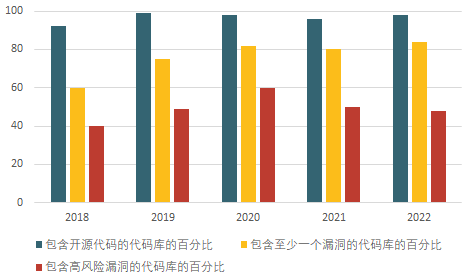
\includegraphics[width=0.75\textwidth]{figures/Proportion}
 \caption{2018-2022年Synopsys审计代码库中的开源代码及漏洞占比示意图}
 \label{fig:Proportion}
\end{figure}
同时,Synopsys统计了包含易受攻击组件的代码库占比,其中使用JQuery 和 Lodash 两个最流行的开源组件的代码库占比达到了47\%和 31\%,其余组件占比如图\ref{fig:assembly}所示。
\begin{figure}
    \centering
    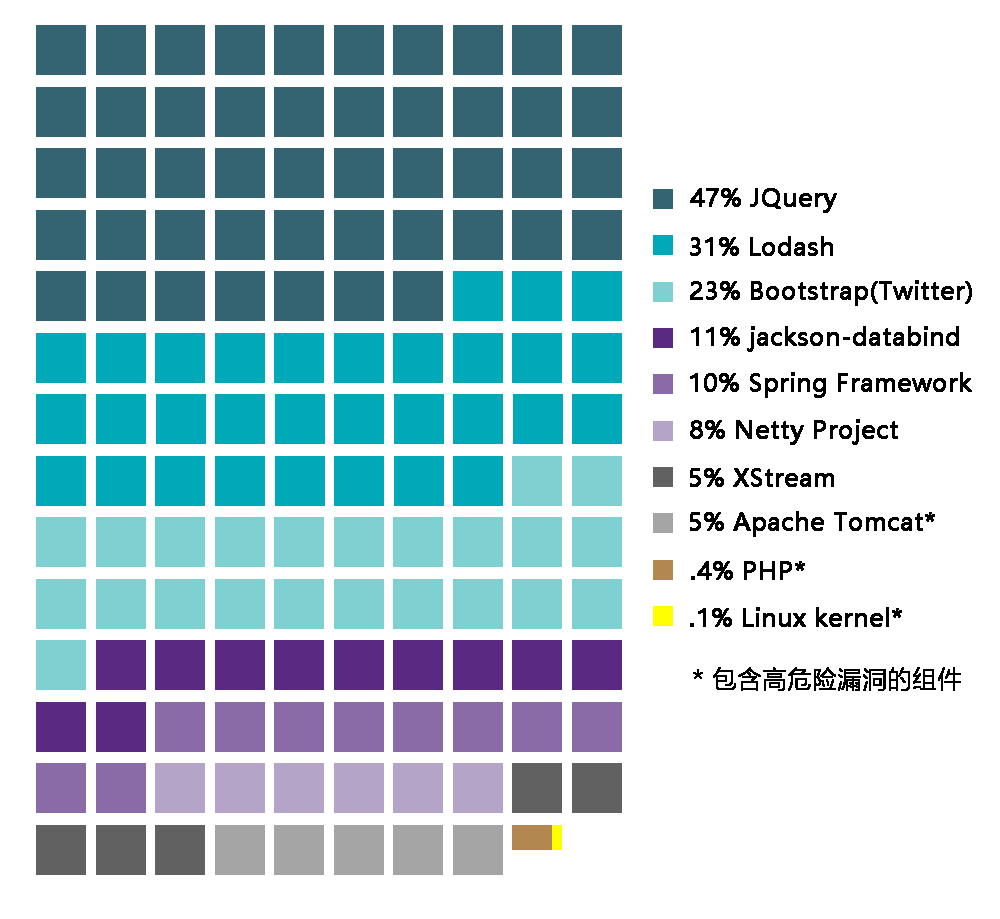
\includegraphics[width=0.75\textwidth]{figures/assembly}
    \caption{2022年Synopsys审计代码库中包含易受攻击组件的百分比示意图}\label{fig:assembly}
\end{figure}
据Gartner\cite{Gartner_2022}预测,到2025年,全球45\%的组织将遭受软件供应链攻击,比2021年增加三倍。因此,准确地检测代码克隆对于软件开发和维护是至关重要的。

早期代码克隆检测技术通常将代码视为自然语言文本进行处理,通过文本相似性判断代码相似程度;随着编译技术的发展,研究者们将编译原理中的词法分析技术运用到代码克隆检测领域;近年来,基于多维源代码表征学习的代码克隆检测技术已经引起了学者们广泛的兴趣,有研究人员从代码克隆检测与代码表征学习技术相结合这一方面进行了探索,试图从关键技术点入手,找到合适的结合点,以提高定代码克隆检测技术的效率和智能化程度。


\section{研究现状与趋势}

\subsection{代码克隆检测技术概述}
%\label{sec:features}
代码克隆检测技术,旨在自动化定位软件系统中的代码克隆,节省成本,减少出错风险,有助于更好地保证软件质量。目前已有的代码克隆方法大多需要对代码片段进行信息抽取,转换为中间表征,然后根据表征方式的不同计算不同代码片段之间的相似度,完成克隆检测任务。其具体流程如图\ref{fig:figure1}所示。
\begin{figure}
    \centering
    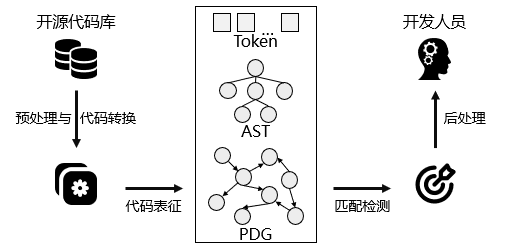
\includegraphics[width=0.95\textwidth]{figures/figure1}
    \caption{代码克隆检测流程}\label{fig:figure1}
\end{figure}

从图\ref{fig:figure1}可以看出一个完整的代码克隆检测过程通常包括预处理、代码转换、表征学习、匹配检测、后处理几个阶段。具体而言,一般的代码克隆检测从代码预处理开始,首先删除与检测无关的空白行、注释、缩进等元素,并根据检测粒度将源代码划分为单独的片段,比如类、函数等;然后将比较单元转化为相应的中间表示,常见的中间表示有:词法单元(Token)、抽象语法树(abstract syntax tree,AST)、程序依赖图(Program dependency graph,PDG)等;在表征学习阶段,将根据上一阶段得到的中间表示采用相应的匹配算法进行相似度计算,例如抽象语法树的比较通常采用子树匹配算法,程序依赖图的比较则采用子图同构算法。此阶段将代码片段两两对比,以查找相似代码源片段,得到代码克隆对。

在这些步骤中,源代码表征方式决定了检测方法的预处理方式、模型设计、部署方式、运行效率,并影响最终结果[2]。

代码克隆检测和代码表征学习之间存在密切的关系。代码表征学习是指利用机器学习或深度学习技术从源代码中学习有效的表示,以便于后续的软件工程任务,如代码克隆检测、代码推荐、缺陷预测等。

在代码克隆检测中,代码表征学习可以用来提取代码片段的特征表示,这些特征表示能够捕捉代码的语法、语义以及结构信息。通过学习到的代码表征,我们可以更准确地比较和识别不同代码片段之间的相似性,从而实现克隆代码的检测和管理。

常见的代码表征学习方法包括基于深度学习的方法,如卷积神经网络(CNN)、循环神经网络(RNN)、注意力机制等。这些方法可以从源代码中学习到高层次的抽象特征表示,使得克隆代码检测可以在更抽象的层次上进行,从而提高检测的准确性和鲁棒性。

因此,代码表征学习为代码克隆检测提供了重要的技术支持,它使得我们能够更有效地利用机器学习和深度学习技术来处理大规模的代码库,并提高代码克隆检测的性能和效率。

因此源代码表征学习是代码克隆检测的关键步骤。

\subsection{代码表征学习}



\section{研究内容}

代码克隆检测是软件工程领域一项重要任务,如何对代码进行合适的表征是代码克隆检测的关键问题。代码表征学习决定了对源代码信息抽取程度的上限,决定了检测技术的预处理方法、模型设计、部署方式、运行效率,并会影响最终结果。面向代码克隆检测这一下游任务,代码表征学习研究存在以下不足:对代码结构信息语义信息利用不充分,特征表达不够完善;表征模型对数据集、模型结构和优化算法等多方面因素的要求高等问题,这些不足严重制约着代码克隆检测技术的发展。因此,研究人员一方面通过对源代码进行充分利用,提出多维源代码表征方法,从而提高代码克隆检测能力;另一方面,通过研究更先进的算法来提高表征模型的自动化和智能化程度,也是目前重要的发展趋势。

本文的主要工作包括:

(1)提出面向代码克隆检测的多维源代码表征学习方法 

针对现有代码表征学习方法存在的对代码结构信息和语义信息利用不充分、表征模型对数据集依赖过高等问题,本文提出面向代码克隆检测的多维源代码表征学习方法,旨在通过构建三个不同维度的代码表征模型,将源代码的语义信息表示为稠密低维实值向量,以在低维空间中高效计算实体和关系的语义联系,并通过特征融合得到多维特征,实现对代码信息的充分利用,以更加全面准确与智能化的方式提高代码克隆测试效率。

(2)面向集外词问题的Token表征学习

具体的,针对Token序列特征挖掘,提出预训练增强辅助模型提取属性特征,从而解决传统基于Token序列的方法存在的集外词问题;
针对抽象语法树AST特征挖掘,提出子树划分的改进方法提取结构特征,从而解决传统基于抽象语法树的方法存在的梯度消失问题;
针对程序依赖图PDG特征挖掘,提出过滤机制提取语义特征,通过收集PDG的简单特征来过滤掉明显不可能为克隆的PDG对,从而解决传统基于程序依赖图的方法存在的计算开销大问题。
针对不同的特征采用不同的代码表征模型对代码片段进行多维源代码特征学习,从而提高对源代码特征提取的程度,并通过特征融合得到一个更能代表代码信息的多维特征,该多维特征能够在低维空间中高效计算实体和关系的语义联系,提高后续代码克隆检测任务的准确率。

(3)实验评估

如图\ref{fig:diagram}所示

\begin{figure}
 \centering
 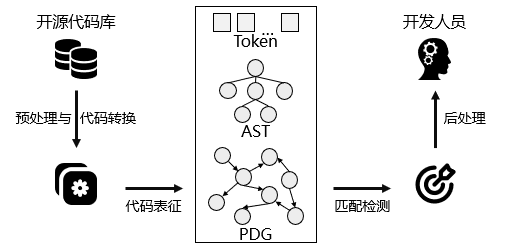
\includegraphics[width=0.75\textwidth]{figures/figure1}
 \caption{热塑性形状记忆聚氨酯的形状记忆机理示意图}\label{fig:diagram}
\end{figure}


\section{论文结构}
%\label{sec:requirements}
本文围绕三个关键技术点展开研究,论文后续各章节具体内容如下:
第1章 绪论 该部分对本文的研究背景与意义进行了阐述 
第2章 从
第3章 介绍基于预训练辅助模型的Token表征学习方法的设计与实现。
第4章 介绍基于子树划分的抽象语法树表征学习方法设计与实现。
第5章 介绍基于图过滤的程序依赖图表征学习方法设计与实现。
第6章 本文研究框架RLCCD的实验验证。
结论 对全文的研究进行了总结,并提出对未来工作的展望。

\cite{Jiang2005Size} ,如表 \ref{tab:category}所示。

%%==================================================
%% chapter02.tex for BIT Master Thesis
%% modified by yang yating
%% version: 0.1
%% last update: Dec 25th, 2016
%%==================================================
\chapter{面向代码克隆检测的多维源代码表征方法}

本章主要介绍代码克隆检测的基本处理流程,分析代码克隆检测过程中的关键技术点及目前存在的挑战,基于此提出本文的面向代码克隆检测的多维源代码表征方法框架的研究方案,并就该框架的设计思路和总体架构进行详细阐述,同时也介绍了该框架包含的3个关键技术点,即基于预训练辅助模型的Token表征学习、基于子树划分的抽象语法树表征学习、基于图过滤的程序依赖图表征学习。

\section{代码克隆检测关键技术}

目前已有的代码克隆检测方法大多遵循以下思路:(1)首先对代码片段进行预处理;(2)对处理好的代码片段进行信息抽取,将其转换为中间表征;(3)根据表征的方式不同计算不同代码片段之间的相似度,完成克隆检测任务。



\section{源代码表征学习的关键技术挑战}



\section{研究方案}
针对上述提出的技术中面临的关键挑战,本文提出面向代码克隆检测的多维源代码表征方法RLCCD。本节首先介绍RLCCD框架的研究思路及总体框架,然后根据流程介绍代码处理、多维源代码表征学习、克隆检测任务实现三个步骤,其中,多维源代码表征学习步骤中分别针对2.2节提出的3个关键挑战提出了对应的解决办法。




\subsection{研究思路及总体框架}

本文围绕三个关键技术点展开研究,论文后续各章节具体内容如下:

\subsection{代码处理}
代码处理的目标是生成源代码片段对应的Token序列、抽象语法树和程序依赖图,主要包含3个流程:抽取代码块、代码标准化、生成中间表示。首先,使用TXL工具从源代码中提取出代码块。这里的源码来自POJ104公共数据基准集,而TXL是专门为软件分析和源代码转换任务设计的一个分析工具,可以很好地支持C语言;然后,对代码块中的代码进行代码标准化处理。具体的,首先需要去除代码块中的注释、空格和空行,然后根据一定的转化规则进行代码标准化;最后,基于标准化后的代码片段生成对应的中间表示:Token序列、抽象语法树AST和程序依赖图PDG。

\subsection{多维源代码表征学习}
RLCCD框架的核心步骤是源代码表征学习,其目标是学习能够表示代码片段的连续向量,表现程序理解的认知层次,获取程序的语法、语义信息,创建程序更高抽象层次上的表示,它决定着对源代码信息抽取程度的上限,决定着检测方法的预处理方式、模型设计、部署方式、运行效率,并影响后续代码克隆检测任务所能检测的精度。下面从Token序列、抽象语法树AST、程序依赖图PDG三种不同维度的代码特征表示出发,详细介绍研究方案并分析其优化改进。

(1)针对Token序列特征挖掘,提出预训练增强辅助模型提取属性特征,从而解决传统基于Token序列的方法存在的集外词问题;

(2)针对抽象语法树AST特征挖掘,提出子树划分的改进方法提取结构特征,从而解决传统基于抽象语法树的方法存在的梯度消失问题;

(3)针对程序依赖图PDG特征挖掘,提出过滤机制提取语义特征,通过收集PDG的简单特征来过滤掉明显不可能为克隆的PDG对,从而解决传统基于程序依赖图的方法存在的计算开销大问题。

(4)特征融合方法
特征融合的目标是将提取到的属性特性、结构特征、语义特征合并,得到一个更能代表代码信息的多维特征,更具有判别能力。

按照具体的技术,特征融合包括特征拼接、特征求和(均值、pooling、加权求和)、特征之间对应元素相乘、特征之间求外积再送入神经网络、跳跃连接(skip)、反卷积、典型相关分析CCA、注意力机制(包括self-attention)加权求和、构图然后采用图神经网络等等。
\subsection{克隆检测任务实现}
克隆检测任务实现的目标是通过计算两个代码的向量距离来判断是否存在代码克隆。常见的向量距离包括欧式距离、曼哈顿距离等。由于代码克隆检测问题是一个二分类问题,即给定两个代码片段,需要输出0或1,0表示它们之间不相似,1表示相似。因此需要将向量距离d映射到0~1之间,这里可以通过sigmoid函数、tanh函数等做映射,其函数值表示两个代码片段的相似度。然后设定阈值,当相似度大于阈值,则判定两个代码片段属于代码克隆,输出1。

\section{本章小结}
本章首先对代码克隆检测的工作流程进行了概述,并分析了源代码表征学习在代码克隆检测过程中所面临的关键技术挑战,主要表现为XXX。针对上述提出的三个问题,提出了本文的方法RLCCD,并介绍了其整体框架和处理流程,对其中的关键技术点进行了简要的论述。




%%==================================================
%% chapter02.tex for BIT Master Thesis
%% modified by yang yating
%% version: 0.1
%% last update: Dec 25th, 2016
%%==================================================
\chapter{基于预训练辅助模型的Token表征学习}
本章主要对本文提出的基于预训练辅助模型的Token表征学习方法进行详细介绍,首先介绍其基本思想,接着阐述其方法设计,以及具体的实现过程,最后介绍实验验证过程和结果。
\section{研究动机}

本文针对现有存在的问题,

基于Token的代码表征通常利用词法分析器将代码中的词汇单元(Token)划分出来。这些词汇单元通常包含关键字、数字、标识符等。将代码表示为词汇单元序列之后,利用深度学习技术对其进行建模,学习代码序列中所包含的有效信息,如功能语义信息、语法结构信息等,最后生成具有丰富代码信息的表征向量,应用于后续的代码克隆检测任务中。现有方法大多都对token进行了规范化,比如将变量名用统一的标识符来代替,这样存在的问题是会丢失部分词法信息,但是如果不进行规范化,会存在集外词(Out-of-vocabulary,简称OOV)的问题,即出现了在词汇表中不存在的token。集外词OOV问题严重限制了代码表示的有效性。

针对上述问题,本文采用预训练增强的辅助模型得到词汇表,从而提高代码克隆检测的准确率。
\section{方法设计}

本节将主要介绍基于预训练辅助模型的Token表征学习方法设计与实现,首先介绍该方法的整体框架,并分别从预训练辅助模型、Token表征学习的具体设计及实现。

\subsection{框架概述}
基于预训练辅助模型的Token表征学习:

\subsection{预训练辅助模型}
Word2vec模型 多次迭代维护词汇表,从而减少OOV问题

在模型训练之前,通过选取合适的模型从代码语料库中学习基本单元的语法语义信息,以及这些单元之间的联系,最终给出一份单词-向量形式的词汇表,从而减少出现集外词问题的概率。具体的,第一次迭代选择相邻的两个token组合为一个单元,查找出最频繁的token组合确定为一个组合单元,并将组合单元更新到词汇表中,然后二次迭代,每次迭代在原来的基本单元上再组合一个新的邻近token作为新的判断单元,每次迭代都会更新词汇表。在得到词汇表之后,根据词汇表获取每个单元的向量表示。
\subsection{Token表征学习}
采用BiLST模型

将token序列对应的向量输入到Bi LSTM网络中,经过Bi LSTM学习哪些信息应该被记住哪些信息应该被遗忘,最终得到每个基本单元包含语义信息和上下文信息的向量表示。Bi LSTM由一个正向的LSTM和一个反向的LSTM组成,主要思想是通过把序列向前、向后分别输入给两个独立的递归网络,这两个子网络连接到一个输出层,在每个词的输出部分把两个子网络的输出信息进行整合,这样网络就同时拥有了序列中每个词的过去时刻信息和未来时刻信息。Bi LSTM可以捕获到序列前后的关系依赖,将代码片段的Token序列转换为可相互比较的向量。
\section{实验验证}
为了验证基于预训练辅助模型的Token表征方法的有效性,

\subsection{实验设计}
(1)实验环境

(2)实验数据集
POJ104数据集

(3)评估指标
分类问题 采用召回率(Recall)、精确度(Precision)和准确率(Accuracy)三个指标评价实验结果

\subsection{预训练辅助模型实验结果}
消融对比实验:体现改进的辅助模型的有效性
基于Token的Bi LSTM
基于Token的+预训练辅助模型的Bi LSTM


\begin{table}
  \centering
  \caption{预训练辅助模型实验结果} \label{tab:category}
  \begin{tabular*}{0.9\textwidth}{@{\extracolsep{\fill}}cccc}
  \toprule
    对比			&P		&R		&F1 \\
  \midrule
    基于Token的Bi LSTM			&0.xx	&0.xx		&0.xx \\
    基于Token的+预训练辅助模型的Bi LSTM			&0.xx		&0.xx		&0.xx \\
  \bottomrule
  \end{tabular*}
\end{table}

\section{本章小结}
本章




%%==================================================
%% chapter02.tex for BIT Master Thesis
%% modified by yang yating
%% version: 0.1
%% last update: Dec 25th, 2016
%%==================================================
\chapter{基于子树划分的抽象语法树表征学习}
本章主要对本文提出的基于子树划分的抽象语法树表征学习方法进行详细介绍,首先介绍其基本思想,其次阐述其具体方法设计与实现,最后进行实验验证。
\section{研究动机}
本文针对现有存在的问题,

抽象语法树AST是源代码语法结构的一种抽象表现形式,以树的形式包含了源代码中的语法信息和语法结构。利用深度神经网络对抽象语法树进行建模得到其向量表示,根据该特征向量完成代码克隆检测任务,实现基于树的源代码表征。现有的方法主要分为两类:一类是将AST转换为完整的二叉树,另一类是将AST直接视作二叉树,这两种方法都会或多或少破坏源代码原有的语法结构,而且在转换的过程会增加AST的高度,AST树过高会导致梯度消失问题,可能会丢失长期上下文信息,削弱了神经模型捕捉更真实和复杂语义的能力。
\section{方法设计}

本节将介绍基于子树划分的抽象语法树表征学习方法设计与实现, 

\subsection{框架概述}
基于子树划分的抽象语法树表征学习:

\subsection{子树划分}
针对上述问题,本文将每个大型的AST分割成小语句树序列,并通过捕获语句的词法和句法知识将每一个语句树都编码成一个向量。
\subsection{抽象语法树表征学习}
在得到一个语句向量序列后,将语句向量序列输入Tree LSTM网络中生成代码片段的结构向量表示。与标准LSTM结构类似,Tree-LSTM神经网络中每个神经元都包括类似的输入门,输出门和隐层输出。不同的是Tree-LSTM单元中门向量和神经元状态的更新依赖于所有与之相关的子单元的状态,另外,Tree-LSTM拥有多个遗忘门,分别对应当前节点的每个子节点,因此 Tree-LSTM可以选择性地从子节点中获取信息,从而保存语义信息更加丰富的子节点的信息。通过Tree LSTM模型,本文能够学习到基于抽象语法树的结构向量,通过这种连续向量表现基于树的理解认知层次,获取程序的结构信息,创建更高抽象层次上的表示,从而提高后续代码克隆检测任务的精度。
\section{实验验证}
为了验证基于子树划分的抽象语法树表征学习方法的有效性,本文
\subsection{实验设计}
和3.3.1 相同
\subsection{抽象语法树子树划分实验结果}
消融对比实验:体现AST子树划分的有效性

基于AST的Tree-LSTM

基于AST的+子树划分的Tree-LSTM

\begin{table}
  \centering
  \caption{抽象语法树子树划分实验结果} \label{tab:category}
  \begin{tabular*}{0.9\textwidth}{@{\extracolsep{\fill}}cccc}
  \toprule
    对比			&P		&R		&F1 \\
  \midrule
    基于AST的Tree-LSTM			&0.xx	&0.xx		&0.xx \\
    基于AST的+子树划分的Tree-LSTM			&0.xx		&0.xx		&0.xx \\
  \bottomrule
  \end{tabular*}
\end{table}

\section{本章小结}
本章




%%==================================================
%% chapter02.tex for BIT Master Thesis
%% modified by yang yating
%% version: 0.1
%% last update: Dec 25th, 2016
%%==================================================
\chapter{基于图过滤的程序依赖图表征学习}
本章主要对本文提出的基于图过滤的程序依赖图表征学习方法进行详细介绍,首先介绍其基本思想,其次阐述其具体方法设计与实现,最后进行实验验证。
\section{研究动机}
本文针对现有存在的问题,

程序依赖图PDG是程序的一种图形表示,所含结构信息最多,能够表示程序的控制依赖,数据依赖以及地址依赖等关系,是一种带有标记的有向多重图。程序依赖图PDG结点代表语句,边代表依赖关系,依赖关系包括数据依赖和控制依赖。通过将程序表示为图的形式使得模型能够更好地理解代码中不同部分之间的依赖关系。现有的方法大多通过图匹配的方法,将PDG图中的控制流和数据流编码为一个紧凑的语义特征矩阵,其中每个元素都是一个高维的稀疏二值特征向量,通过寻找矩阵之间的相似模式来判定克隆代码。但这些方法通常需要消耗大量的时间和空间,计算开销大。
\section{方法设计}
本节将介绍基于图过滤的程序依赖图表征学习方法设计与实现, 

\subsection{框架概述}
基于图过滤的程序依赖图表征学习:

\subsection{图过滤机制}
针对上述问题,本课题引入过滤机制,通过收集PDG的简单特征来过滤掉明显不可能为克隆的PDG对。具体的,根据PDG的节点个数、控制边数、执行边数、数据边数、声明节点数、函数调用数、传入参数、传出参数等代表特征进行过滤,在大幅减少候选PDG对规模的同时,保证真正的克隆对不会被过滤掉而导致整体克隆检出率的降低。

\subsection{程序依赖图表征学习}
对于提取到的程序依赖图,本课题拟通过图卷积神经网络将其转换成向量。图卷积神经网络是一种特殊的前馈神经网络结构,为减少网络中参数个数,用卷积层来代替传统的全连接层,提高神经网络的训练效率,卷积神经网络可以提取信息最多的数据特征,生成一个固定大小的向量表示结构,从而挖掘深层次的语法和语义信息,在代码克隆检测任务中有较好的性能表现。
\section{实验验证}
为了验证基于图过滤的程序依赖图表征学习方法的有效性,本文
\subsection{实验设计}
和3.3.1 相同
\subsection{图过滤机制实验结果}
消融对比实验:体现图过滤机制的有效性

基于PDG的GCN

基于PDG的+图过滤的GCN


\begin{table}
  \centering
  \caption{图过滤机制实验结果} \label{tab:category}
  \begin{tabular*}{0.9\textwidth}{@{\extracolsep{\fill}}cccc}
  \toprule
    对比			&P		&R		&F1 \\
  \midrule
    基于PDG的GCN			&0.xx	&0.xx		&0.xx \\
    基于PDG的+图过滤的GCN			&0.xx		&0.xx		&0.xx \\
  \bottomrule
  \end{tabular*}
\end{table}

\section{本章小结}
本章




%%==================================================
%% chapter02.tex for BIT Master Thesis
%% modified by yang yating
%% version: 0.1
%% last update: Dec 25th, 2016
%%==================================================
\chapter{多维源代码表征方法RLCCD整体框架}
本章主要对面向代码克隆检测的多维源代码表征方法整体框架RLCCD进行介绍,同时进行实验评估及验证。具体地,RLCCD是由上述基于预训练辅助模型的Token表征学习、基于子树划分的抽象语法树表征学习、基于图过滤的程序依赖图表征学习方法三种维度融合形成并进行实现的表征方法,最后通过与SourcererCC、ASTNN、SCDetector进行对比实验以验证该框架的有效性。
\section{特征融合}
特征融合
\section{实验设置}
本文的实验设计主要围绕以下4 个方面的研究问题:

• RQ1:本文提出的预训练辅助模型策略是否优于基线方法?(见3.3 节)

• RQ2:本文提出的子树划分策略是否优于基线方法?(见4.3 节)

• RQ3:本文提出的图过滤策略能否优于基线方法?(见5.3 节)

• RQ4:与现有代码克隆检测工具相比,RLCCD 表现如何?

\subsection{实验环境}
(1)系统环境

本章实验均在Ubuntu 16.04 LTS(64位)系统下进行。


\subsection{实验数据集}
本章实验部分采用的数据集为代码克隆检测领域常见的基准集POJ104,该数据集是一个基于C语言构建的大型数据集,包含了104个编程问题以及学生提交的对应问题的不同C语言源代码,在该数据集中,针对同一问题的不同源解法的代码被视为一个克隆对。

首先通过筛选,得到51485个源代码样本,然后随机生成50000个代码克隆对,其中包含5200个真克隆对,44800个假克隆对。依据随机种子将数据集按照3:1:1划分为训练集、测试机、验证集,其中的正负样本数如下表。


\subsection{对比工具}
在对比整个方法的效果时,本文选取开源的SourcererCC、ASTNN、SCDetector方法进行比较。

SourcererCC:SourcererCC是一种相对较新的基于token的克隆检测工具。该工具通过词袋模型,把收集的数据全部编码成词频信息,后将代码行转换成一个由词频构成的向量,通过向量的比较获取相似度。

ASTNN:一种基于神经网络的源代码表示方法。它将整个抽象语法树AST分解成一系列小型语句子树,并通过捕获语句的词法和语法信息将语句子树分别编码为向量,最后采用了RNN模型生成代码片段的向量表示。ASTNN方法完整保留了抽象语法树的结构信息,能够检测到所有类型的代码克隆。

SCDetector:是基于令牌和基于图的方法的结合。给定一个方法源代码,我们首先生成CFG,然后应用中心性分析将图转换为某些语义标记(即具有图细节的标记)。最后,这些语义标记被馈送到Siamese网络中,以训练模型并使用它来检测代码克隆对。

\section{RLCCD框架评估 }

对比实验:体现框架的有效性


\begin{table}
  \centering
  \caption{RLCCD实验结果} %\label{tab:category}
  \begin{tabular*}{0.9\textwidth}{@{\extracolsep{\fill}}cccc}
  \toprule
    对比			&P		&R		&F1 \\
  \midrule
    SourcererCC			&0.xx	&0.xx		&0.xx \\
    ASTNN			&0.xx		&0.xx		&0.xx \\
    SCDetector			&0.xx	&0.xx		&0.xx \\
    RLCDD			&0.xx		&0.xx		&0.xx \\
  \bottomrule
  \end{tabular*}
\end{table}

\section{本章小结}
本章节主要对RLCCD框架进行了实验验证,以验证RLCCD的XXX能力。




%%==================================================
%% conclusion.tex for BIT Master Thesis
%% modified by yang yating
%% version: 0.1
%% last update: Dec 25th, 2016
%%==================================================


\begin{conclusion}

尽管模糊测试在漏洞挖掘方面取得了较好的成果,但其仍存在一定的随机性和盲目性,受限于生成种子的效率和质量。近年来,研究人员从模糊测试与智能化技术相结合这一方面进行了探索,试图从关键技术点入手,找到合适的结合点,以提高模糊测试技术的效率和智能化程度。

\end{conclusion}

%% 参考文献,五号字,使用 BibTeX,包含参考文献文件.bib

\bibliography{reference/chap1}
%\bibliography{reference/chap1,reference/chap2} %多个章节的参考文献



%%%%%%%%%%%%%%%%%%%%%%%%%%%%%%
%% 后置部分
%%%%%%%%%%%%%%%%%%%%%%%%%%%%%%

%% 附录(章节编号重新计算,使用字母进行编号)
%\appendix
%\renewcommand\theequation{\Alph{chapter}--\arabic{equation}}  % 附录中编号形式是"A-1"的样子
%\renewcommand\thefigure{\Alph{chapter}--\arabic{figure}}
%\renewcommand\thetable{\Alph{chapter}--\arabic{table}}

%%%==================================================
%% app1.tex for BIT Master Thesis
%% modified by yang yating
%% version: 0.1
%% last update: Dec 25th, 2016
%%==================================================


\chapter{***}

附录相关内容…
 
%
\chapter{Maxwell Equations}


因为在柱坐标系下,$\overline{\overline\mu}$是对角的,所以Maxwell方程组中电场$\bf
E$的旋度

所以$\bf H$的各个分量可以写为:
\begin{subequations}
  \begin{eqnarray}
    H_r=\frac{1}{\mathbf{i}\omega\mu_r}\frac{1}{r}\frac{\partial
      E_z}{\partial\theta } \\
    H_\theta=-\frac{1}{\mathbf{i}\omega\mu_\theta}\frac{\partial E_z}{\partial r}
  \end{eqnarray}
\end{subequations}
同样地,在柱坐标系下,$\overline{\overline\epsilon}$是对角的,所以Maxwell方程组中磁场$\bf
H$的旋度
\begin{subequations}
  \begin{eqnarray}
    &&\nabla\times{\bf H}=-\mathbf{i}\omega{\bf D}\\
    &&\left[\frac{1}{r}\frac{\partial}{\partial
        r}(rH_\theta)-\frac{1}{r}\frac{\partial
        H_r}{\partial\theta}\right]{\hat{\bf
        z}}=-\mathbf{i}\omega{\overline{\overline\epsilon}}{\bf
      E}=-\mathbf{i}\omega\epsilon_zE_z{\hat{\bf z}} \\
    &&\frac{1}{r}\frac{\partial}{\partial
      r}(rH_\theta)-\frac{1}{r}\frac{\partial
      H_r}{\partial\theta}=-\mathbf{i}\omega\epsilon_zE_z
  \end{eqnarray}
\end{subequations}
由此我们可以得到关于$E_z$的波函数方程:
\begin{eqnarray}
  \frac{1}{\mu_\theta\epsilon_z}\frac{1}{r}\frac{\partial}{\partial r}
  \left(r\frac{\partial E_z}{\partial r}\right)+
  \frac{1}{\mu_r\epsilon_z}\frac{1}{r^2}\frac{\partial^2E_z}{\partial\theta^2}
  +\omega^2 E_z=0
\end{eqnarray}
 

%(其后部分无编号)
\backmatter

% 发表文章目录
%%==================================================
%% pub.tex for BIT Master Thesis
%% modified by yang yating
%% version: 0.1
%% last update: Dec 25th, 2016
%%==================================================

\begin{publications}{99}

    \item\textsc{高凌}. {交联型与线形水性聚氨酯的形状记忆性能比较}[J].
      化工进展, 2006, 532-535.(核心期刊)
    
\end{publications}

% 致谢
%%==================================================
%% thanks.tex for BIT Master Thesis
%% modified by yang yating
%% version: 0.1
%% last update: Dec 25th, 2016
%%==================================================

\begin{thanks}

本论文的工作是在导师……。

\end{thanks}

% 作者简介(博士论文需要)
%%%==================================================
%% resume.tex for BIT Master Thesis
%% modified by yang yating
%% version: 0.1
%% last update: Dec 25th, 2016
%%==================================================

\begin{resume}

本人…。

\end{resume}


\end{document}
